\chapter{Introduction}

%What does manifacturing mean?
\begin{quotation}
    \noindent
    \textsf{\textit{Manifacturing} is a word which is derived from Latin and it means \textit{made by hand}. This is suited to a reality where most commercial goods where totally made by hand. After many years, factory appeared and the way the products were made changed a lot! In particular the attention was on the use of \textit{machines} instead of \textit{handcrafted mehtods}. In the modern era machines, people and processes to handle them are grouped in complex \textit{production systems} that not rarely are \textbf{automated} and \textbf{computerized}.  
    }
\end{quotation}

\section{Production systems}
A \textbf{production system} is a compound of people, machine, procedures whose aim is to \textit{perform the manifacturing operations} of a firm. Any production system can be divided in two basic components: 
\begin{description}
    \itemsep-0.2em
    \item[\textsc{Facilities}] they consist of the factory (physical structure), machines, material handling and inspection equipments and all computer systems to control the manifacturing operations. The \textbf{plant layout} is included in this part and is related to the way equipment and workers are \textit{arranged} into the factory. Machines and general equipment are divide into \textbf{manifacturing systems} that are groups of machines to carry out some operations fort the production. Roughly speaking, they are all the components that "touch" the products.
    \item[\textsc{Manifacturing support systems}]  These are all the procedure used by the company to manage production and to solve all the problems related to it. In this branch are included product design, the planning of the manifacturing and some control and business operations.
\end{description}
\noindent
The  \Cref{fig:prod_sys_structure} shows schematically what we have just briefly explained here. Along this notes the scheme will be gradually enriched by other topics. 

\begin{figure}
    \centering
    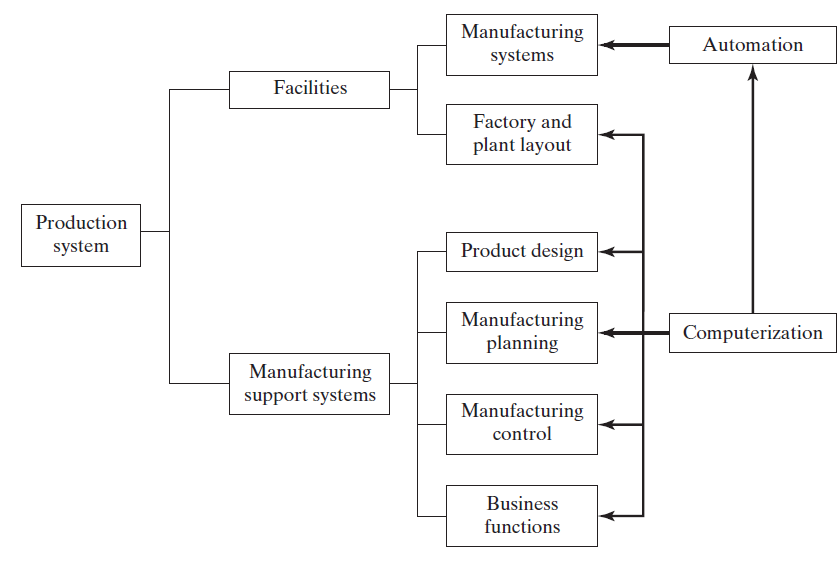
\includegraphics[scale=0.8]{img/prod_system_scheme.png}
    \caption{Production system structure and types of automation}
    \label{fig:prod_sys_structure}
\end{figure}

\section{Automation in production systems}
\textbf{Automation} refers to the possibility to substitute human through machines in order to execute different works. Mainly two types of automation on machines can be considered: (i) \textit{semiautomated machine} which execute only a part of the task independently; (ii) \textit{fully automated machine} is capable to work for long period without the human attention.\\
Some components of the production system are prone to be automated while other tasks require to operated manually. Also in these case we can divide such components in two categories:
\begin{enumerate}
    \itemsep-0.3em
    \item \textsf{\textbf{Automation} of the manifacturing systems}
    \item \textsf{\textbf{Computerization} of the manifacturing support systems}
\end{enumerate}

\subsection{Automated manifacturing systems}
Three basic types of automation can be distinguished that practically operates as fully automated systems.
\subsubsection{Fixed automation}
The sequence of processing operation is \textit{fixed} in the equipment configuration. If there is a sequence of operations to be performed they are usually simple, or they are combination of simple tasks. Such type of systems are used when there is the necessity to produce large quantities of pieces. They are suitable especially when there is small variations in the products.
\subsubsection{Programmable automation}
At the opposite, we find the \textbf{programmable automation}. Here there is the possibility to change the sequence of operations. The sequence of operations is dictated by a \textbf{program} which is a sequence of instructions written so that they can be interpreted by the system. They are used for low quantities and for batch production. Note that to produce a new batch of a different item: (i) we have to rewrite the program; (ii) we have to change the setup for equipments. This requires a \textit{changeover time}. Instances of programmable automation are Numerical controlled (NC) machines and Programmable logical controllers (PLCs).

\subsubsection{Flexible automation}
Such a type of automation is an extension of the previous with the difference that the changeover time is virtually avoided. What makes \textit{flexibility} possible is the fact that the differences between processed parts are not significant, so the changeover necessity is "little". Manifacturing systems which performs machinery processes are in this category.

\subsection{Computerized manifacturing support systems}
Automating the part of the production system devoted to manifacturing support is in order to reduce the manual and clerical required effort. In this context the term \textbf{Computer Integrated Manifacturing (CIM)} refers to the pervasive use of computers to \textit{design products}, \textit{plan the production}, \textit{control the operations} and so on. Other terms are used to indicate components of the CIM, in particular the \textit{Computer Aided Design (CAD)} supports the the design of the product, while \textit{Computer-Aided manifacturing (CAM)} is used for functions related to the planning.\\

A core operation in automation is \textbf{control}, which can be practically carried out using an \textbf{open-loop procedure} (or \textit{feedforward}) or in a \textbf{closed-loop} fashion, which exploting the negative feedback principle makes the overall system capable to correct the actions to be performed. Such a type of control strategy is used in the great majority of the application, this is why we focus on automation system which are based on them.

\subsection{Closed-loop automation system}
A \textbf{closed-loop automation system} can be divided into three subsystems: (i) Instrumentation subsystem, (ii) Control subsystem, (iii) Human-interface subsystem.

\begin{figure}[h]
    \centering
    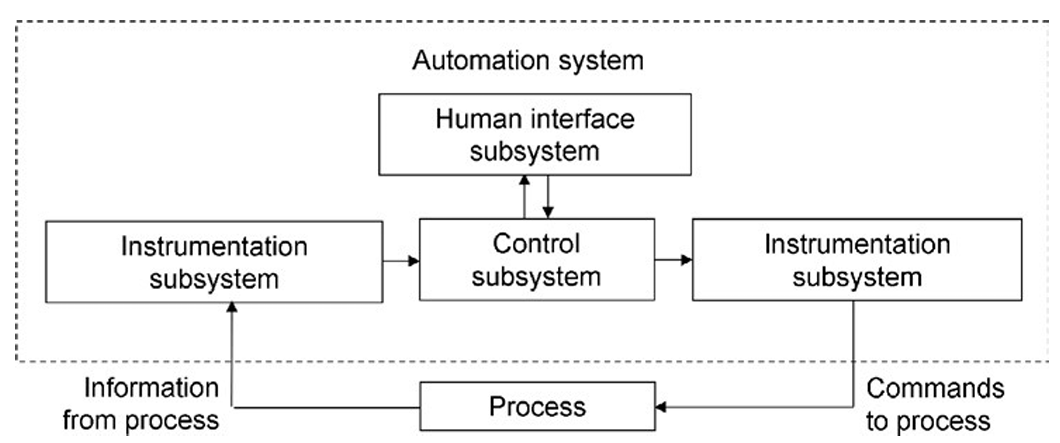
\includegraphics[scale=0.5]{img/closed_loop_automation.png}
\end{figure}

\subsubsection{i) Instrumentation subsystem}
Is the part devoted to the acquirement of information related to the behaviour of the process (by measuring its variables), such measurements are then sent to a conditioning circuit and then to the control subsystem. \\ 
The instrumentation devices (practically \textbf{sensors}) have different structures according to the input and output signals to be measured. They can be both analog or digital. Moreover they can be classified as \textbf{transducer} if their output is sent over short distances, \textbf{transmitter} if the output signal is sent over long distances.

\subsubsection{ii) Control subsystem}
It is the heart of any closed-loop automated system and it is in charge for carrying out several (basic) functions regarding: 
\begin{itemize}
    \itemsep-0.3em
    \item \textsf{Instrumentation subsystem}, in particular measured variables are compared to reference values in order to steer the control action through a certain direction by using again the instrumentation; 
    \item \textsf{Human Interface subsystem}, in particular the associated information are an input of the control part which through the instrumentation sends information to the process.
\end{itemize}
Other advanced tasks of control systems are: i) \textit{safety monitorning} in which some sensors are used in order to track potentially dangerous operations; ii) \textit{maintenance and repair diagnostic} in which the system assists in identifying the source of potential failures; iii) \textit{error detection and recovery} the error detection step uses the available sensor to pick data, classify the error and adopt the needed operation so that the system could achieve again the normal status.

\subsubsection{iii) Human-Interface subsystem}
The \textbf{Human interface} is very important since allows the human to interact with the process in order to change its behaviour. Anyway, if a manual change is not needed the operator can observe it and eventually steer the direction of the process being carried out. The interaction between humans and the process is done essentially by using \textbf{valves/breakings} in order to force the process going through a certain direction.

\begin{figure}
    \centering
    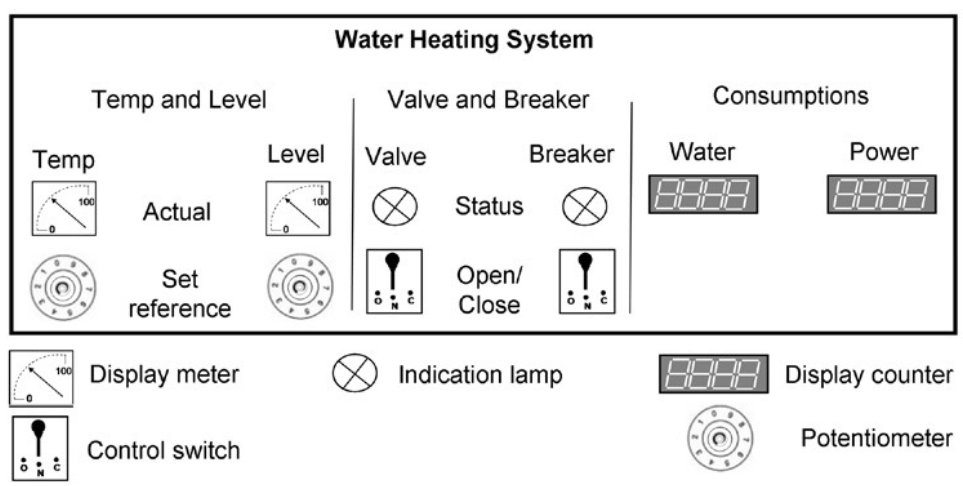
\includegraphics[scale=0.5]{img/hmi.png}
    \caption{Human-Machine Interface}
\end{figure}

\subsubsection{\textsc{How computers are involved in control}}
Computers can be used in automating production systems in different modalities. In the following we propose a brief review.
\begin{description}
    \item[\textsf{Continuous control}] Here the objective is \textit{keep the value of an output value at a certain desired level} (clearly this concept can be extended, in the sense that in industrial field many different variables can be \textbf{regulated}). Such a type of controllers can be implemented through \textbf{embedded systems} (mostly operational amplifiers, resistors and capacitors). An example could be the control of the output of a chemical reaction. To be more specific we can distinguish the following tipologies of continuous control: 
    \begin{itemize}
        \itemsep-0.3em
        \item \textbf{Regulatory control} where the objective is to maintain the process performacnce within a given tolerance, a compensating action is taken whether there is an output which is different than the desired one (that is the same to state that thee is a non-zero reference tracking error).
        \item \textbf{Feedback-Feedforward control} In presence of disturbances a feedforward controller can be introduced in order to sense and compensate its effect;
        \item \textbf{Adaptive control} It is particularly useful in order to control time-variant systems or to control systems in a time-variant environment. After having identified what are the varied variables, and what should be changed into the control, a modification is implemented.
    \end{itemize}
    \item[\textsf{Discrete control}] In this case the variables of the system are changed at discrete time, moreover also the action to be performed are discrete typically ON/OFF decisions. This type of control is implemented by using \textbf{PLCs}. This can be event driven (the system state is changed) or time-driven (a certain amount of time is spent).
\end{description}

\begin{remark} 
    \textit{Continuous control strategies} can be also implemented by using digital controllers. In this case the controller is put in an A/D/A chain in order to properly convert relevant signals. By using the digital control approach one is able to perform more complex control actions, think about input constraints, nonlinearities and so on.
\end{remark}

To conclude this paragraph we provide a glossary with some important concept together with their definition.

\begin{table}[h]
    \centering
    \begin{tabular}{p{5cm} p{10cm}}
        \toprule
        \textbf{Numerical control}&{Concerns the use of a computers or a microcontroller in order to control a  \textit{machine tool} by using a program with a sequence of operations (see G-Code)}\\
        \midrule
        \textbf{Programmable Logic Controllers (PLCs)}&{They were introduced in the 70s to substitute electromechanical relays, they can be programmed in order to perform timing, sequencing and counting operations}\\
        \midrule
        \textbf{Supervisory control}&{It is applied to an higher level than the process, and the objective is to optimize some well-defined function}\\
        \midrule
        \textbf{Distributed control systems}&{It is made up of a communication network between computers and PLCs in order to distribute as much as possible the process workload}. In this context there is a central control room in which Supervisory control happens and local operator stations are present in ordet to introduce redundancy.\\
        \bottomrule
    \end{tabular}
\end{table}

\section{Levels of automation}
We have seen that a production system is the composition of different subsystems than can be themselves automated, this is the same to say that in a factory we can talk about automation at different levels. 
\begin{enumerate}
    \itemsep-0.3em
    \item \emph{Device level} Is the lowest level and it is made up of the different components of a single machine. For example at device level we have the feedback loop controlling a single manipulator arm;
    \item \emph{Machine level} Putting together all the parts of a device, control happens at machine level. Typical actions at this stage are performing some basic functions described by a program. 
    \item \emph{Cell level or system level} A cell is nothing but a group of machines connected each other by a computer to which is associated a certain function for the manifacturing system. Typical control functions are the coordination between different machines in order to perform a certain task.
    \item \emph{Plant level} This is the factory or production system level and it receives instructions from the enterprise level and translate them into process planning, purchasing and quality control. At this level control is implemented by using a \textbf{SCADA (Supervisory control and Data Acquisition)} which: (i) displays the current state of the process; (ii) displays alarms and error logs; displays the trends analyzing them.
    \item \emph{Enterprise level} the control actions at this stage are in order to manage the company.
\end{enumerate}

What is interesting to analyzein this form of hierarchy is that \textit{the higher the level, the longest the response time with respect to the control actions}. Moreover the decisions are less but more complicated ones, the same holds for the quantity of informations that flows from one level to another.


\begin{figure}
    \centering
    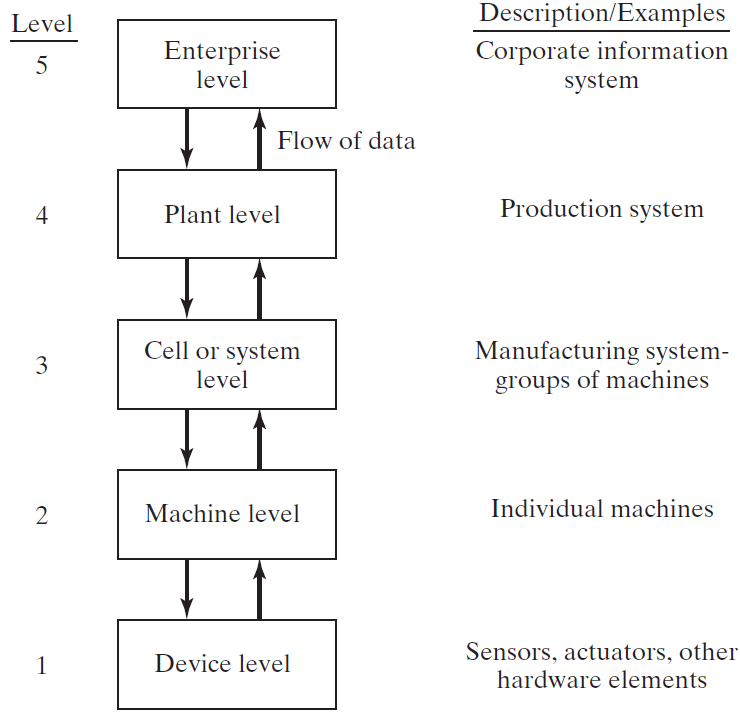
\includegraphics[scale=0.6]{img/automation_level.png}
    \caption{Different levels of automation}
\end{figure}

\section{Operation and Process Databases}
In an automated production system, some databases are used in order to store relevant information about the single operations or the process. 

\begin{figure}[h]
    \centering
    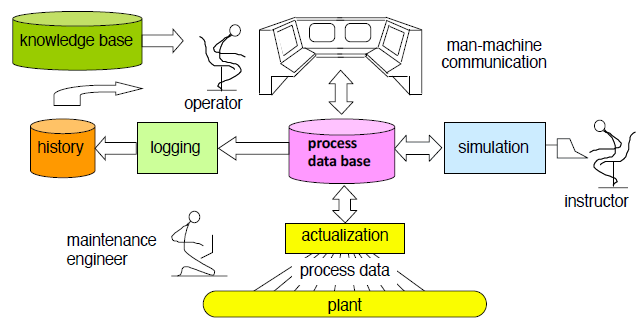
\includegraphics[scale=0.9]{img/Databases.png}
    \caption{Databases in automated manifacturing system}
    \label{fig:Databases}
\end{figure}

The \Cref{fig:Databases} shows the interactions between the different parts of the automated production system and the databases themselves. We can distinguish:
\begin{itemize}
    \itemsep-0.3em
    \item \textsf{Process Database} this keeps the latest known states of the plant (the granularity of the tracked operations are of the order of the day, hour or minute);
    \item \textsf{Historical Database} registers snapshot (namely \texttt{VIEW}) from the historical database capturing what happened to the plant in a given period (eg. a bimester, a semester...)
    \item \textsf{Knowledge Database} Is the most particular database which comprises a mixture of process and history data in order to track solved issues, trouble-shooting procedures, documentation and so on.
\end{itemize}

In order to conclude this chapter we present an example of automated industrial production system, highlighting the different levels of automation and used devices and protocols (\textit{ABB Industrial IT}).

\begin{figure}[h]
    \centering
    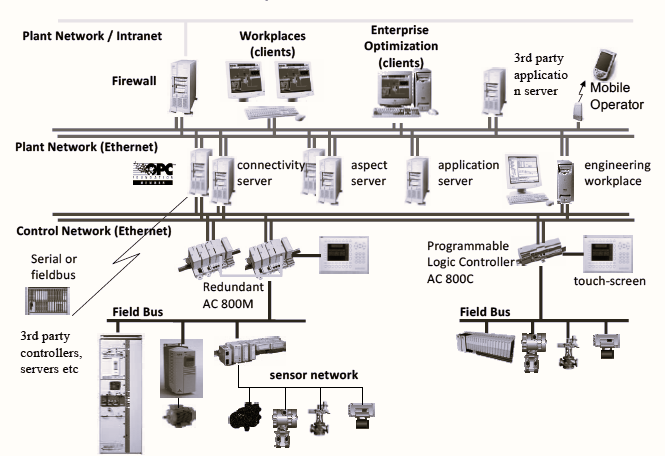
\includegraphics[scale=0.9]{img/ABB.png}
    \caption{ABB Industrial IT}
\end{figure}